% Define the type of document.
\documentclass[12pt, a4paper]{article}

% Set a more sensible document size.
\usepackage[margin=0.75in]{geometry}

% Set the language.
\usepackage[british]{babel}
    \usepackage{csquotes}

% Prevent words from being split accross lines.
\tolerance=1\emergencystretch=\maxdimen\hyphenpenalty=10000\hbadness=10000

% Allows images to be included.
\usepackage{graphicx}
    \graphicspath{ {./images/} }

% Allow disabling of floating objects.
\usepackage{float}

% Sets the title.
\title{Computer Graphics: Geometry and Simulation\\Coursework 2: Simulation}
\author{Oliver Jones (s2153980)}
\date{}

% Begin the document.
\begin{document}
\maketitle

This report makes references to videos, which can be found in the
    \texttt{videos} directory of the submission.
The relevant files are named accordingly within the report.

The code for sections 1 and 2 can be found in the \texttt{section-12} directory
    of the submission, containing the \texttt{scene.h} and \texttt{mesh.h} files.
The code for section 3 can be found in the \texttt{section-3} directory,
    containing the same mesh.h and constraints.h files, with an updated version of
    the scene.h file.
All other files from the original codebase remain unchanged.

\section{Linear FEM Matrices \& Constrained Time Integration}
    % Detail insights on the results (and artifacts and advantages and disadvantages) of linear FEM on the existing scenes.
    % Encouraged to generate new scenes to demonstrate your insights more clearly.
    \paragraph{}
        The linear FEM method works well for small deformations, with no noticeable
            artefacts occurring, as seen in \texttt{bunny-12.mov}, which depicts
            \texttt{bunny-scene.txt}.
        In contrast, \texttt{epcot-12.mov} and \texttt{cube86-12.mov}, depicting
            \texttt{epcot-scene.txt} and \texttt{cube86-scene.txt} respectively,
            demonstrate clear artefacts when larger deformations are involved.
        The cubes in \texttt{cube86-12.mov} end up massively sheared and stretched,
            with the artefacts becoming more pronounced as the simulation progresses.
        Meanwhile, in \texttt{epcot-12.mov}, the Epcot model becomes stretched and
            flattened as the simulation progresses.

\section{Extension: Corotational Elements}
    % Demonstrate the difference clearly, which should be evident where big deformations are involved.
    \paragraph{}
        Two very obvious improvements can be seen with \texttt{cube86-scene.txt} in
            \texttt{cube86-3.mov}, and \texttt{epcot-scene.txt} in \texttt{epcot-3.mov}.
        The cubes in \texttt{cube86-3.mov} no longer become sheared or stretched, and
            the Epcot model in \texttt{epcot-3.mov} no longer becomes stretched or
            flattened.

    \paragraph{}
        Figure~\ref{fig:cube86} shows the difference between the resting states of
            linear FEM and corotational elements for the cube scene.
        The corotational elements maintain the cube's shape, while the linear FEM
            elements do not.

    \paragraph{}
        Figure~\ref{fig:epcot} shows the difference between the resting states of
            linear FEM and corotational elements for the Epcot scene.
        Once again, the corotational elements maintain the Epcot model's shape, while
            the linear FEM elements do not.

    \paragraph{}
        On the other hand, \texttt{fertility-scene.txt} shows relatively little
            difference between linear FEM and corotational elements, as seen in
            \texttt{fertility-12.mov} and \texttt{fertility-3.mov}.

    \paragraph{}
        \begin{figure}[H]
            \centering
            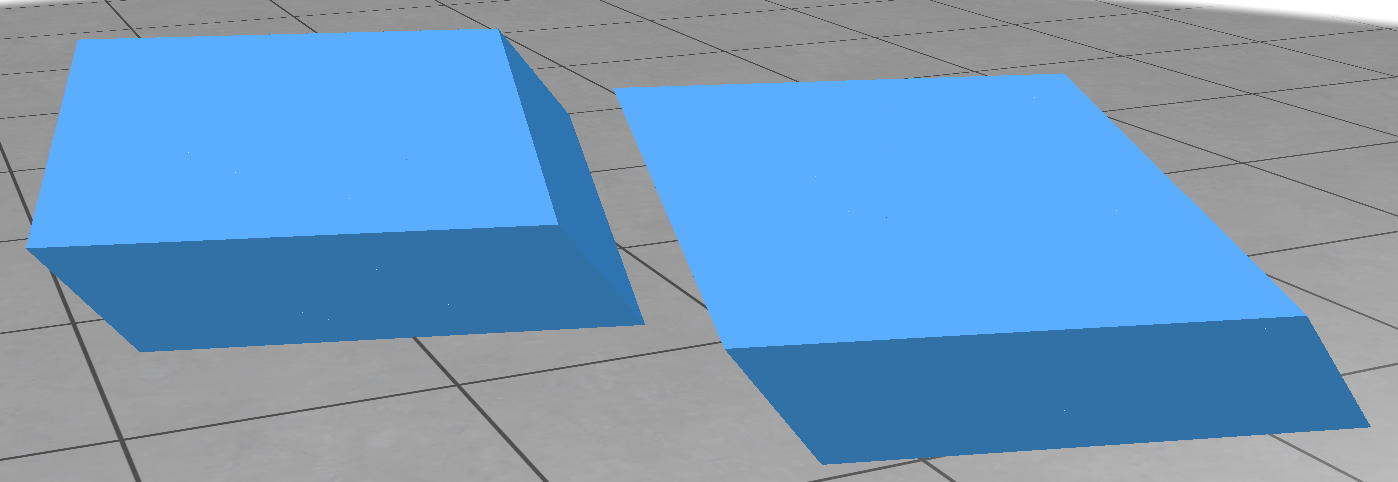
\includegraphics[width=\textwidth]{cube86-12.png}
            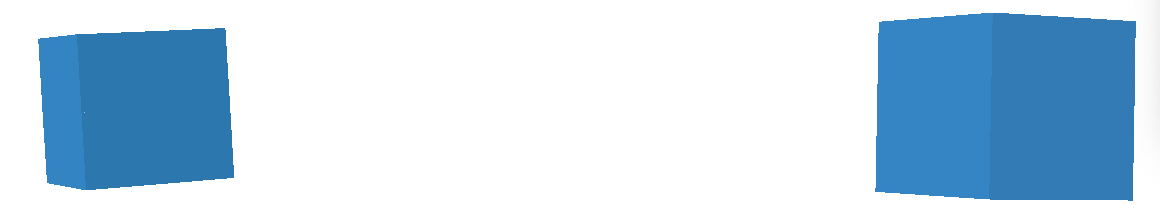
\includegraphics[width=\textwidth]{cube86-3.png}
                \caption{Comparison of linear FEM (top) and corotational elements (bottom) for the cube scene.}
                \label{fig:cube86}
        \end{figure}

        \begin{figure}[H]
            \centering
            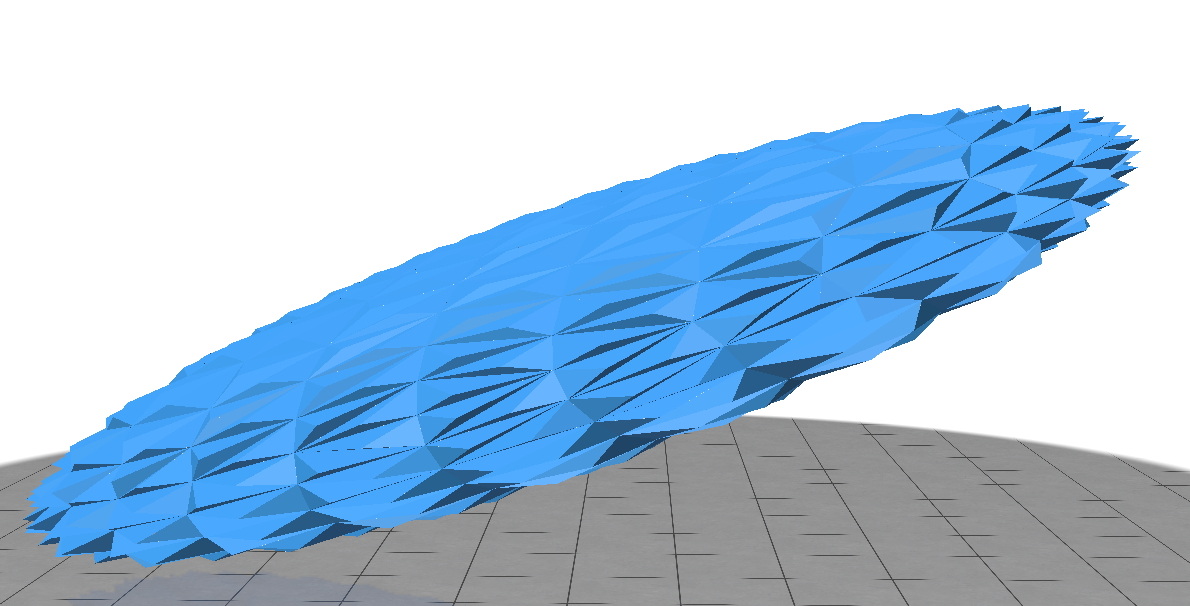
\includegraphics[width=0.49\textwidth]{epcot-12.png}
            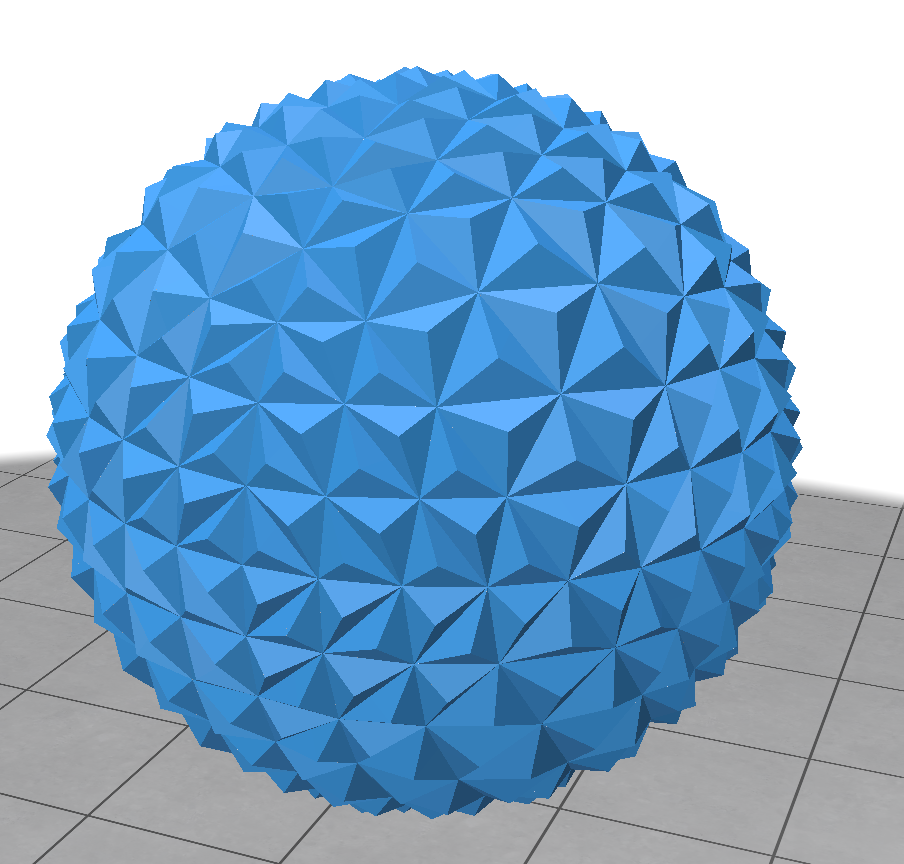
\includegraphics[width=0.49\textwidth]{epcot-3.png}
                \caption{Comparison of linear FEM (left) and corotational elements (right) for the Epcot scene.}
                \label{fig:epcot}
        \end{figure}

    \paragraph{}
        Despite the improvements in many cases, it comes at a cost.
        The corotational elements are much more computationally expensive.
        This is most noticeable in the \texttt{epcot-scene.txt} simulation, where the
            frame rate drops significantly when using corotational elements, which can be
            seen in \texttt{epcot-3.mov}, compared to \texttt{epcot-12.mov}.

\end{document}
